\chapter{\ifproject%
\ifcpe การทดลองและผลลัพธ์\else Experimentation and Results\fi
\else%
\ifcpe การประเมินระบบ\else System Evaluation\fi
\fi}

การประเมินระบบสำหรับโครงงานนี้จะเน้นไปที่การคำนวณค่าความเหมาะสมของตารางสอบที่ได้จากระบบ เพื่อเปรียบเทียบกับตารางสอบที่กำหนดโดยสำนักทะเบียนและประมวลผล 
\enskip การคำนวณค่าความเหมาะสมของตารางสอบที่ได้นั้นจะคำถึงนึงคุณสมบัติของตารางสอบตามวัตถุประสงค์ของโครงงาน ดังที่ได้ระบุไว้ในตอนที่~\ref{sec:Objectives} 
โดยสามารถประเมินความเหมาะสมได้ 2 วิธี กล่าวคือ การนับจำนวนครั้งที่ตารางสอบสำหรับนักศึกษาคนใดๆ ไม่เป็นไปตามที่พึงประสงค์ และการสอบถามความพึงพอใจของนักศึกษาที่มีต่อตารางสอบที่ได้จากระบบ เพื่อช่วยในการยืนยันว่าตัวชี้วัดที่โปรแกรมใช้คำนวณค่าความเหมาะสมของตารางสอบนั้นสอดคล้องกับความต้องการของผู้ใช้งานอย่างแท้จริง

\section{การประเมินระบบด้วย penalty}
การประเมินผลระบบจัดตารางสอบที่จะพัฒนาขึ้นมานั้นจะพิจารณาปัจจัยด้านความสมดุลและความเหมาะสมของตารางสอบที่ได้ โดยสามารถกำหนดค่าอันไม่พึงประสงค์ (penalty) ของตารางสอบแต่ละแบบที่เป็นผลลัพธ์จากระบบ
\enskip ตารางสอบที่มีความเหมาะสมมาก ควรจะมี penalty น้อย
\enskip นอกจากจะมีการคำนวณ penalty เพื่อเปรียบเทียบตารางสอบแบบต่างๆ ที่ได้จากระบบแล้ว การคำนวณในลักษณะเดียวกันนี้จะใช้กับตารางสอบดั้งเดิมดังที่ได้กำหนดโดยสำนักทะเบียนและประมวลผลอีกด้วย เพื่อยืนยืนว่าตารางสอบที่ได้จากระบบนั้นมีคุณภาพดีกว่าตารางสอบที่มีอยู่เดิม

\subsection{การคำนวณ penalty}
Penalty ของตารางสอบแต่ละแบบที่ได้จากระบบนั้น คำนวณได้จากค่า penalty ของการที่มีนักศึกษาที่สอบในช่วงเวลาใด ๆ ที่เกินกว่าจํานวนที่นั่งสอบที่ทางมหาวิทยาลัยสามารถจัดให้ได้
รวมกับค่า penalty ของตารางสอบสำหรับนักศึกษารายบุคคล ว่ามีความเหมาะสมกับนักศึกษารายนั้นๆ มากน้อยเพียงใด 
โดยการคิดค่า penalty ของนักศึกษาแต่ละคนนั้น จะใช้ตัวชี้วัดทั้งสิ้น 6 แบบ ซึ่งมีน้ำหนักแตกต่างกันไปตามความไม่พึงประสงค์ที่สรุปได้จากผลสำรวจ
โดยคิดจากสัดส่วนนักศึกษาที่ไม่ชอบให้เกิดสถานการณ์ดังกล่าว ซึ่งได้กำหนดให้มีค่า Penalty ของสถานการณ์ต่าง ๆ ที่เกิดขึ้นในตารางสอบของนักศึกษาแต่ละคน เรียงตามน้ำหนักจากมากไปน้อยได้ดังนี้
  
\begin{enumerate}
    \item จํานวนนักศึกษาเกินความจุที่นั่งสอบของคณะ มีการคิดค่า penalty ตามที่จะกล่าวต่อไป
    \item มีนักศึกษาคนใด ๆ ถูกกำหนดให้สอบสองวิชาในเวลาเดียวกัน ครั้งละ 10000 Points
    \item มีนักศึกษาคนใด ๆ ถูกกำหนดให้สอบเวลา 8.00--11.00\,น. และ 12.00--15.00\,น. ในวันเดียวกัน ครั้งละ 78 Points
    \item มีนักศึกษาคนใด ๆ ถูกกำหนดให้สอบเวลา 12.00--15.00\,น. และ 15.30--18.30\,น. ในวันเดียวกัน ครั้งละ 78 Points
    \item มีนักศึกษาคนใด ๆ ถูกกำหนดให้สอบเวลา 8.00--11.00\,น. และ 15.30--18.30\,น. ในวันเดียวกัน ครั้งละ 38 Points
    \item มีนักศึกษาคนใด ๆ ถูกกำหนดให้สอบเวลา 15.30--18.30\,น. และ 08.00--11.00\,น. ในวันรุ่งขึ้น ครั้งละ 29 Points
    \item นักศึกษามีวันเว้นว่างระหว่างการสอบสองวิชาที่ติดกันมากกว่า 3 วัน ครั้งละ 12 Points
\end{enumerate}
สำหรับค่า Penalty ที่เกิดจากจำนวนนักศึกษาเกินความจุที่นั่งสอบของคณะในแต่ละช่วงเวลาสอบนั้นจะมีการคิดคำนวณแยกตามคณะดังนี้
\begin{itemize}
    \item หากจัดให้นักศึกษาสอบที่คณะแล้วจำนวนนักศึกษารวมมากกว่า 100\% ของที่นั่งสอบในคณะสำหรับวิชาของคณะนั้น ๆ ในแต่ละช่วงเวลาที่สอบ จะจัดให้นักศึกษาสอบเต็ม 80\% ของที่นั่งคณะ
    หลังจากนั้นจัดให้นักศึกษาที่เกินความจุ 80\% สอบที่ตึกอาคารเรียนรวมเท่าที่จัดได้หากอาคารเรียนรวมยังมีที่นั่งเหลือ แต่หากจัดที่อาคารเรียนรวมแล้วยังมีที่นั่งไม่เพียงพอ จะทำการคิดค่า penalty ของนักศึกษาที่เหลือ
    โดยหากจำนวนนักศึกษาเกินความจุ 80\% ไป แต่ไม่เกิน 100 \% จะคิดตามสมการเส้นตรงดังนี้ 
    \begin{equation}
        f(x)=500(x-80)
    \end{equation}
    หากจำนวนนักศึกษาเกินความจุ 100 \% จะคิดตามสมการเอกซ์โพเนนเชียลดังนี้ 
    \begin{equation}
        f(x)=500(x-80)+2^{2(\frac{x}{10}-1)}-2^{18}
    \end{equation}
    โดยที่ค่า x คือ เปอร์เซ็นต์ของความจุที่นั่งของคณะที่ใช้ไปแล้ว
    \item หากจัดให้นักศึกษาสอบที่คณะแล้วจำนวนนักศึกษารวมมากกว่า 80\% ของที่นั่งสอบในคณะสำหรับวิชาของคณะนั้น ๆ ในแต่ละช่วงเวลาที่สอบ แต่ไม่เกิน 100\% จะจัดให้นักศึกษาสอบเต็ม 80\% ของที่นั่งคณะ
    หลังจากนั้นจัดให้นักศึกษาที่เกินความจุ 80\% สอบที่ตึกอาคารเรียนรวมเท่าที่จัดได้หากอาคารเรียนรวมยังมีที่นั่งเหลือ แต่หากจัดที่อาคารเรียนรวมแล้วยังมีที่นั่งไม่เพียงพอ จะทำการคิดค่า penalty ของนักศึกษาที่เหลือแต่เกิน 80\% ไป
    โดยคิดตามสมการเส้นตรงที่ 4.1
    \item หากจัดให้นักศึกษาสอบที่คณะแล้วจำนวนนักศึกษารวมไม่เกิน 80\% ของที่นั่งสอบในคณะสำหรับวิชาของคณะนั้น ๆ ในแต่ละช่วงเวลาที่สอบ จะไม่มีการคิด penalty
    \item สุดท้ายคิด penalty ของอาคารเรียนรวม หากจำนวนนักศึกษารวมที่ต้องสอบที่อาคารเรียนรวมเกิน 80\% แต่ไม่เกิน 100\% จะคิดตามสมการเส้นตรงที่ 4.1 แต่หากจำนวนนักศึกษารวมที่ต้องสอบที่อาคารเรียนรวมเกิน 100\% จะคิดตามสมการเอกซ์โพเนนเชียลที่ 4.2
\end{itemize}
ค่า penalty จะค่อย ๆ เพิ่มขึ้นหลังจากจำนวนนักศึกษารวมเกิน 80\% ของที่นั่งสอบขึ้นไป และเริ่มเพิ่มขึ้นอย่างรวดเร็วหากจำนวนนักศึกษาเกิน 100\% ของที่นั่งสอบดังกราฟที่ \ref{fig:penalty_graph}
\begin{figure}
    \begin{center}
      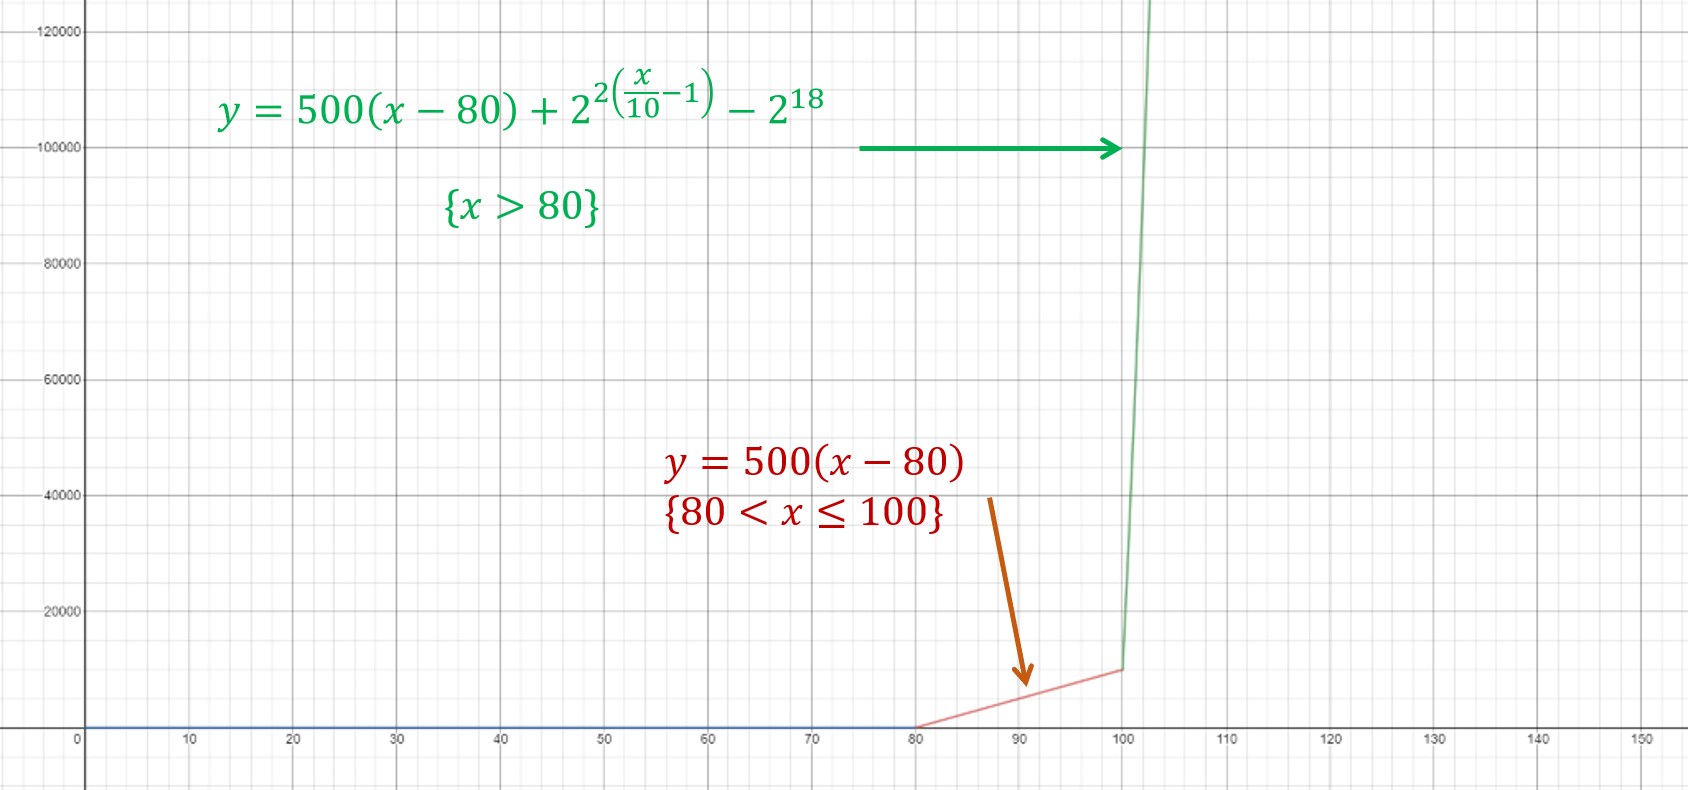
\includegraphics[width=\linewidth]{images/penalty_graph.png}
    \end{center}
    \caption[กราฟแสดงการเพิ่มขึ้นของค่า penalty]{กราฟแสดงการเพิ่มขึ้นของค่า penalty}
    \label{fig:penalty_graph}     
\end{figure}
\newpage
\section{การประเมินระบบโดยสอบถามความพึงพอใจของนักศึกษา}
ตัวชี้วัดที่ใช้ในการคำนวณ penalty ของตารางสอบที่ได้จากระบบนั้น อาจจะไม่ครอบคลุมความพึงประสงค์ทุกรูปแบบจากนักศึกษา หรือน้ำหนักของตัวชี้วัดที่ใช้ในการคำนวณ penalty นั้นอาจจะเป็นไปได้หลายรูปแบบ
\enskip การสอบถามความพึงพอใจของนักศึกษานั้นจะช่วยในการปรับปรุงอัลกอริทึมเพื่อให้สามารถเลือกใช้น้ำหนักของตัวชี้วัดที่เหมาะสมมากขึ้นในการจัดตารางสอบ
อีกทั้งยังช่วยยืนยันว่าตัวชี้วัดที่โปรแกรมใช้คํานวณค่าความเหมาะสมของตารางสอบนั้นสอดคล้องกับความต้องการของผู้ใช้งาน 
\enskip โดยการประเมินระบบด้วยวิธีการนี้นั้นจะมีการแสดงตารางสอบหลายแบบเพื่อให้นักศึกษาได้เปรียบเทียบและ
ให้คะแนนความพึงพอใจกับตารางสอบแบบต่าง ๆ ซึ่งตารางสอบที่ใช้ในแบบสอบถามนั้นจะเป็นตารางสอบของนักศึกษาคนที่ตอบแบบสอบถาม 
โดยเป็นตารางสอบที่มีค่า penalty ต่ำที่สุดที่ได้จากระบบ โดยจะมีตารางสอบหลายแบบที่มีค่าน้ำหนักของตัวชี้วัดที่แตกต่างกันออกไป 
และรวมไปถึงตารางสอบดั้งเดิมของสำนักทะเบียนและประมวลผลด้วย

\section{ผลการประเมินระบบด้วยค่า penalty}
การประเมินระบบด้วยค่า penalty นั้นได้มีการจัดตารางสอบทั้งหมด 6 ภาคการศึกษา ตั้งแต่ภาคการศึกษาที่ 1/2561 จนถึงภาคการศึกษาที่ 2/2563
โดยในแต่ละภาคการศึกษาได้มีการทดลองจัดตารางสอบด้วยอัลกอลิทึมทั้งหมด 4 รูปแบบ และได้คิดคำนวณจำนวนครั้งที่เกิด penalty และค่า penalty ของตารางสอบแต่ละแบบ ดังตารางที่ \ref{tab:result_table_161} - \ref{tab:result_table_263}
\begin{table}[]
    \centering
    \textbf{Total courses: 1432} \quad \quad \textbf{Total students having an exam: 13171}
    \resizebox{\textwidth}{!}{%
    \begin{tabular}{@{}ccrrrrrrrr@{}}
    \toprule
    \textbf{รูปแบบ}                              & \textbf{Penalty}                      & \textbf{1}                & \textbf{2}               & \textbf{3}                   & \textbf{4}                  & \textbf{5}                  & \textbf{6}                  & \textbf{7}                    & \textbf{รวม}                  \\ \midrule
                                                 & \textbf{Count}                        & 0                         & 0                        & 354                          & 430                         & 1854                        & 171                         & 12930                         & 15739                         \\ \cmidrule(l){2-10} 
    \multirow{-2}{*}{BFS-DEG}                    & \textbf{Value}                        & 0                         & 0                        & 27612                        & 33540                       & 70452                       & 4959                        & 155160                        & 291723                        \\ \midrule
                                                 & \textbf{Count}                        & 1                         & 0                        & 480                          & 140                         & 207                         & 71                          & 12038                         & 12937                         \\ \cmidrule(l){2-10} 
    \multirow{-2}{*}{DEG}                        & \textbf{Value}                        & 21                        & 0                        & 37440                        & 10920                       & 7866                        & 2059                        & 144456                        & 202762                        \\ \midrule
                                                 & \textbf{Count}                        & 1                         & 0                        & 588                          & 210                         & 93                          & 69                          & 10465                         & 11426                         \\ \cmidrule(l){2-10} 
    \multirow{-2}{*}{BFS-STD}                    & \textbf{Value}                        & 2                         & 0                        & 45864                        & 16380                       & 3534                        & 2001                        & 125580                        & 193361                        \\ \midrule
    {\color[HTML]{FE0000} }                      & {\color[HTML]{FE0000} \textbf{Count}} & {\color[HTML]{FE0000} 1}  & {\color[HTML]{FE0000} 0} & {\color[HTML]{FE0000} 431}   & {\color[HTML]{FE0000} 116}  & {\color[HTML]{FE0000} 174}  & {\color[HTML]{FE0000} 60}   & {\color[HTML]{FE0000} 8334}   & {\color[HTML]{FE0000} 9116}   \\ \cmidrule(l){2-10} 
    \multirow{-2}{*}{{\color[HTML]{FE0000} STD}} & {\color[HTML]{FE0000} \textbf{Value}} & {\color[HTML]{FE0000} 64} & {\color[HTML]{FE0000} 0} & {\color[HTML]{FE0000} 33618} & {\color[HTML]{FE0000} 9048} & {\color[HTML]{FE0000} 6612} & {\color[HTML]{FE0000} 1740} & {\color[HTML]{FE0000} 100008} & {\color[HTML]{FE0000} 151090} \\ \bottomrule
    \end{tabular}%
    }
    \caption{ตารางแสดงค่า penalty ของตารางสอบเทอม 1/2561}
    \label{tab:result_table_161}
\end{table}
\begin{table}[]
    \centering
    \textbf{Total courses: 1551} \quad \quad \textbf{Total students having an exam: 13095}
    \resizebox{\textwidth}{!}{%
    \begin{tabular}{@{}ccrrrrrrrr@{}}
    \toprule
    \textbf{รูปแบบ}                              & \textbf{Penalty}                      & \textbf{1}                  & \textbf{2}               & \textbf{3}                   & \textbf{4}                   & \textbf{5}                   & \textbf{6}                  & \textbf{7}                    & \textbf{รวม}                  \\ \midrule
                                                 & \textbf{Count}                        & 1                           & 0                        & 1050                         & 583                          & 296                          & 314                         & 10977                         & 13221                         \\ \cmidrule(l){2-10} 
    \multirow{-2}{*}{BFS-DEG}                    & \textbf{Value}                        & 2467                        & 0                        & 81900                        & 45474                        & 11248                        & 9106                        & 131724                        & 281919                        \\ \midrule
                                                 & \textbf{Count}                        & 1                           & 0                        & 884                          & 264                          & 398                          & 242                         & 12158                         & 13947                         \\ \cmidrule(l){2-10} 
    \multirow{-2}{*}{DEG}                        & \textbf{Value}                        & 238                         & 0                        & 68952                        & 20592                        & 15124                        & 7018                        & 145896                        & 257820                        \\ \midrule
                                                 & \textbf{Count}                        & 1                           & 0                        & 1343                         & 374                          & 742                          & 208                         & 10342                         & 13010                         \\ \cmidrule(l){2-10} 
    \multirow{-2}{*}{BFS-STD}                    & \textbf{Value}                        & 2                           & 0                        & 104754                       & 29172                        & 28196                        & 6032                        & 124104                        & 292260                        \\ \midrule
    {\color[HTML]{FE0000} }                      & {\color[HTML]{FE0000} \textbf{Count}} & {\color[HTML]{FE0000} 1}    & {\color[HTML]{FE0000} 0} & {\color[HTML]{FE0000} 814}   & {\color[HTML]{FE0000} 247}   & {\color[HTML]{FE0000} 266}   & {\color[HTML]{FE0000} 203}  & {\color[HTML]{FE0000} 9649}   & {\color[HTML]{FE0000} 11180}  \\ \cmidrule(l){2-10} 
    \multirow{-2}{*}{{\color[HTML]{FE0000} STD}} & {\color[HTML]{FE0000} \textbf{Value}} & {\color[HTML]{FE0000} 2251} & {\color[HTML]{FE0000} 0} & {\color[HTML]{FE0000} 63492} & {\color[HTML]{FE0000} 19266} & {\color[HTML]{FE0000} 10108} & {\color[HTML]{FE0000} 5887} & {\color[HTML]{FE0000} 115788} & {\color[HTML]{FE0000} 216792} \\ \bottomrule
    \end{tabular}%
    }
    \caption{ตารางแสดงค่า penalty ของตารางสอบเทอม 2/2561}
    \label{tab:result_table_261}
\end{table}
\begin{table}[]
    \centering
    \textbf{Total courses: 1729} \quad \quad \textbf{Total students having an exam: 19786}
    \resizebox{\textwidth}{!}{%
    \begin{tabular}{@{}ccrrrrrrrr@{}}
    \toprule
    \textbf{รูปแบบ}                              & \textbf{Penalty}                      & \textbf{1}                  & \textbf{2}               & \textbf{3}                   & \textbf{4}                   & \textbf{5}                   & \textbf{6}                  & \textbf{7}                    & \textbf{รวม}                  \\ \midrule
                                                 & \textbf{Count}                        & 0                           & 0                        & 1110                         & 657                          & 1217                         & 639                         & 18036                         & 21659                         \\ \cmidrule(l){2-10} 
    \multirow{-2}{*}{BFS-DEG}                    & \textbf{Value}                        & 0                           & 0                        & 86580                        & 51246                        & 46246                        & 18531                       & 216432                        & 419035                        \\ \midrule
                                                 & \textbf{Count}                        & 1                           & 0                        & 1155                         & 242                          & 522                          & 147                         & 18859                         & 20926                         \\ \cmidrule(l){2-10} 
    \multirow{-2}{*}{DEG}                        & \textbf{Value}                        & 714                         & 0                        & 90090                        & 18876                        & 19836                        & 4263                        & 226308                        & 360087                        \\ \midrule
                                                 & \textbf{Count}                        & 1                           & 0                        & 1500                         & 595                          & 259                          & 159                         & 15990                         & 18504                         \\ \cmidrule(l){2-10} 
    \multirow{-2}{*}{BFS-STD}                    & \textbf{Value}                        & 2                           & 0                        & 117000                       & 46410                        & 9842                         & 4611                        & 191880                        & 369745                        \\ \midrule
    {\color[HTML]{FE0000} }                      & {\color[HTML]{FE0000} \textbf{Count}} & {\color[HTML]{FE0000} 3}    & {\color[HTML]{FE0000} 0} & {\color[HTML]{FE0000} 965}   & {\color[HTML]{FE0000} 334}   & {\color[HTML]{FE0000} 337}   & {\color[HTML]{FE0000} 231}  & {\color[HTML]{FE0000} 15535}  & {\color[HTML]{FE0000} 17405}  \\ \cmidrule(l){2-10} 
    \multirow{-2}{*}{{\color[HTML]{FE0000} STD}} & {\color[HTML]{FE0000} \textbf{Value}} & {\color[HTML]{FE0000} 4259} & {\color[HTML]{FE0000} 0} & {\color[HTML]{FE0000} 75270} & {\color[HTML]{FE0000} 26052} & {\color[HTML]{FE0000} 12806} & {\color[HTML]{FE0000} 6699} & {\color[HTML]{FE0000} 186420} & {\color[HTML]{FE0000} 311506} \\ \midrule
                                                 & \textbf{Count}                        & 0                           & 3247                     & 3406                         & 2333                         & 7663                         & 5863                        & 18667                         & 41179                         \\ \cmidrule(l){2-10} 
    \multirow{-2}{*}{สำนักทะเบียน}                  & \textbf{Value}                        & 0                           & 32470000                 & 265668                       & 181974                       & 291194                       & 170027                      & 224004                        & 33602867                      \\ \bottomrule
    \end{tabular}%
    }
    \caption{ตารางแสดงค่า penalty ของตารางสอบเทอม 1/2562}
    \label{tab:result_table_162}
\end{table}
\begin{table}[]
    \centering
    \textbf{Total courses: 1828} \quad \quad \textbf{Total students having an exam: 19505}
    \resizebox{\textwidth}{!}{%
    \begin{tabular}{@{}ccrrrrrrrr@{}}
    \toprule
    \textbf{รูปแบบ}                              & \textbf{Penalty}                      & \textbf{1}                 & \textbf{2}               & \textbf{3}                    & \textbf{4}                   & \textbf{5}                   & \textbf{6}                  & \textbf{7}                    & \textbf{รวม}                  \\ \midrule
                                                 & \textbf{Count}                        & 1                          & 0                        & 1624                          & 1072                         & 1460                         & 883                         & 16578                         & 21618                         \\ \cmidrule(l){2-10} 
    \multirow{-2}{*}{BFS-DEG}                    & \textbf{Value}                        & 11907                      & 0                        & 126672                        & 83616                        & 55480                        & 25607                       & 198936                        & 502218                        \\ \midrule
                                                 & \textbf{Count}                        & 1                          & 0                        & 1045                          & 374                          & 262                          & 138                         & 19168                         & 20988                         \\ \cmidrule(l){2-10} 
    \multirow{-2}{*}{DEG}                        & \textbf{Value}                        & 545                        & 0                        & 81510                         & 29172                        & 9956                         & 4002                        & 230016                        & 355201                        \\ \midrule
                                                 & \textbf{Count}                        & 0                          & 0                        & 1732                          & 864                          & 785                          & 448                         & 16085                         & 19914                         \\ \cmidrule(l){2-10} 
    \multirow{-2}{*}{BFS-STD}                    & \textbf{Value}                        & 0                          & 0                        & 135096                        & 67392                        & 29830                        & 12992                       & 193020                        & 438330                        \\ \midrule
    {\color[HTML]{FE0000} }                      & {\color[HTML]{FE0000} \textbf{Count}} & {\color[HTML]{FE0000} 1}   & {\color[HTML]{FE0000} 0} & {\color[HTML]{FE0000} 1303}   & {\color[HTML]{FE0000} 250}   & {\color[HTML]{FE0000} 343}   & {\color[HTML]{FE0000} 192}  & {\color[HTML]{FE0000} 14545}  & {\color[HTML]{FE0000} 16634}  \\ \cmidrule(l){2-10} 
    \multirow{-2}{*}{{\color[HTML]{FE0000} STD}} & {\color[HTML]{FE0000} \textbf{Value}} & {\color[HTML]{FE0000} 497} & {\color[HTML]{FE0000} 0} & {\color[HTML]{FE0000} 101634} & {\color[HTML]{FE0000} 19500} & {\color[HTML]{FE0000} 13034} & {\color[HTML]{FE0000} 5568} & {\color[HTML]{FE0000} 174540} & {\color[HTML]{FE0000} 314773} \\ \midrule
                                                 & \textbf{Count}                        & 1                          & 4732                     & 3908                          & 2608                         & 5757                         & 5157                        & 18698                         & 40861                         \\ \cmidrule(l){2-10} 
    \multirow{-2}{*}{สำนักทะเบียน}                  & \textbf{Value}                        & 24129                      & 47320000                 & 304824                        & 203424                       & 218766                       & 149553                      & 224376                        & 48445072                      \\ \bottomrule
    \end{tabular}%
    }
    \caption{ตารางแสดงค่า penalty ของตารางสอบเทอม 2/2562}
    \label{tab:result_table_262}
\end{table}
\begin{table}[]
    \centering
    \textbf{Total courses: 1894} \quad \quad \textbf{Total students having an exam: 26549}
    \resizebox{\textwidth}{!}{%
    \begin{tabular}{@{}ccrrrrrrrr@{}}
    \toprule
    \textbf{รูปแบบ}                              & \textbf{Penalty}                      & \textbf{1}                  & \textbf{2}               & \textbf{3}                    & \textbf{4}                   & \textbf{5}                   & \textbf{6}                  & \textbf{7}                    & \textbf{รวม}                  \\ \midrule
                                                 & \textbf{Count}                        & 2                           & 0                        & 1717                          & 681                          & 511                          & 524                         & 21515                         & 24950                         \\ \cmidrule(l){2-10} 
    \multirow{-2}{*}{BFS-DEG}                    & \textbf{Value}                        & 5633                        & 0                        & 133926                        & 53118                        & 19418                        & 15196                       & 258180                        & 485471                        \\ \midrule
                                                 & \textbf{Count}                        & 2                           & 0                        & 1722                          & 673                          & 506                          & 511                         & 22860                         & 26274                         \\ \cmidrule(l){2-10} 
    \multirow{-2}{*}{DEG}                        & \textbf{Value}                        & 6568                        & 0                        & 134316                        & 52494                        & 19228                        & 14819                       & 274320                        & 501745                        \\ \midrule
                                                 & \textbf{Count}                        & 2                           & 0                        & 1722                          & 654                          & 486                          & 293                         & 23154                         & 26311                         \\ \cmidrule(l){2-10} 
    \multirow{-2}{*}{BFS-STD}                    & \textbf{Value}                        & 3856                        & 0                        & 134316                        & 51012                        & 18468                        & 8497                        & 277848                        & 493997                        \\ \midrule
    {\color[HTML]{FE0000} }                      & {\color[HTML]{FE0000} \textbf{Count}} & {\color[HTML]{FE0000} 2}    & {\color[HTML]{FE0000} 0} & {\color[HTML]{FE0000} 1556}   & {\color[HTML]{FE0000} 681}   & {\color[HTML]{FE0000} 563}   & {\color[HTML]{FE0000} 286}  & {\color[HTML]{FE0000} 20888}  & {\color[HTML]{FE0000} 23976}  \\ \cmidrule(l){2-10} 
    \multirow{-2}{*}{{\color[HTML]{FE0000} STD}} & {\color[HTML]{FE0000} \textbf{Value}} & {\color[HTML]{FE0000} 1252} & {\color[HTML]{FE0000} 0} & {\color[HTML]{FE0000} 121368} & {\color[HTML]{FE0000} 53118} & {\color[HTML]{FE0000} 21394} & {\color[HTML]{FE0000} 8294} & {\color[HTML]{FE0000} 250656} & {\color[HTML]{FE0000} 456082} \\ \midrule
                                                 & \textbf{Count}                        & 0                           & 4983                     & 3786                           & 3498                           & 8676                           & 7784                   & 26703                         & 55430                         \\ \cmidrule(l){2-10} 
    \multirow{-2}{*}{สำนักทะเบียน}                  & \textbf{Value}                        & 0                           & 49830000                 & 295308                         & 272844                         & 329688                         & 225736                 & 320436                        & 51274012                      \\ \bottomrule
    \end{tabular}%
    }
    \caption{ตารางแสดงค่า penalty ของตารางสอบเทอม 1/2563}
    \label{tab:result_table_163}
\end{table}
\begin{table}[]
    \centering
    \textbf{Total courses: 1770} \quad \quad \textbf{Total students having an exam: 24392}
    \resizebox{\textwidth}{!}{%
    \begin{tabular}{@{}ccrrrrrrrr@{}}
    \toprule
    \textbf{รูปแบบ}                              & \textbf{Penalty}                      & \textbf{1}               & \textbf{2}               & \textbf{3}                    & \textbf{4}                   & \textbf{5}                   & \textbf{6}                   & \textbf{7}                    & \textbf{รวม}                  \\ \midrule
                                                 & \textbf{Count}                        & 1                        & 0                        & 2537                          & 747                          & 666                          & 616                          & 22015                         & 26582                         \\ \cmidrule(l){2-10} 
    \multirow{-2}{*}{BFS-DEG}                    & \textbf{Value}                        & 4                        & 0                        & 197886                        & 58266                        & 25308                        & 17864                        & 264180                        & 563508                        \\ \midrule
    {\color[HTML]{FE0000} }                      & {\color[HTML]{FE0000} \textbf{Count}} & {\color[HTML]{FE0000} 1} & {\color[HTML]{FE0000} 0} & {\color[HTML]{FE0000} 1709}   & {\color[HTML]{FE0000} 711}   & {\color[HTML]{FE0000} 693}   & {\color[HTML]{FE0000} 575}   & {\color[HTML]{FE0000} 21042}  & {\color[HTML]{FE0000} 24731}  \\ \cmidrule(l){2-10} 
    \multirow{-2}{*}{{\color[HTML]{FE0000} DEG}} & {\color[HTML]{FE0000} \textbf{Value}} & {\color[HTML]{FE0000} 1} & {\color[HTML]{FE0000} 0} & {\color[HTML]{FE0000} 133302} & {\color[HTML]{FE0000} 55458} & {\color[HTML]{FE0000} 26334} & {\color[HTML]{FE0000} 16675} & {\color[HTML]{FE0000} 252504} & {\color[HTML]{FE0000} 484274} \\ \midrule
                                                 & \textbf{Count}                        & 1                        & 0                        & 2011                          & 1612                         & 743                          & 474                          & 24440                         & 29281                         \\ \cmidrule(l){2-10} 
    \multirow{-2}{*}{BFS-STD}                    & \textbf{Value}                        & 4                        & 0                        & 156858                        & 125736                       & 28234                        & 13746                        & 293280                        & 617858                        \\ \midrule
                                                 & \textbf{Count}                        & 0                        & 1                        & 1862                          & 717                          & 515                          & 342                          & 21313                         & 24750                         \\ \cmidrule(l){2-10} 
    \multirow{-2}{*}{STD}                        & \textbf{Value}                        & 0                        & 10000                    & 145236                        & 55926                        & 19570                        & 9918                         & 255756                        & 496406                        \\ \midrule
                                                 & \textbf{Count}                        & 2                        & 4128                     & 3224                          & 6477                         & 7468                         & 4206                         & 25640                         & 51145                         \\ \cmidrule(l){2-10} 
    \multirow{-2}{*}{สำนักทะเบียน}               & \textbf{Value}                          & 333067582                 & 41280000                 & 251472                        & 505206                       & 283784                       & 121974                       & 307680                        & 375817698                     \\ \bottomrule
    \end{tabular}%
    }
    \caption{ตารางแสดงค่า penalty ของตารางสอบเทอม 2/2563}
    \label{tab:result_table_263}
\end{table}
\begin{table}[]
    \centering
    \resizebox{\textwidth}{!}{%
    \begin{tabular}{@{}cccccc@{}}
    \toprule
                               & \multicolumn{5}{c}{Total Counts of}                                                                                                         \\ \cmidrule(l){2-6} 
    \multirow{-2}{*}{Semester} & \cellcolor[HTML]{F8696B}-2 & \cellcolor[HTML]{FAB2B5}-1 & \cellcolor[HTML]{FCFCFF}0 & \cellcolor[HTML]{B0DDBD}1 & \cellcolor[HTML]{63BE7B}2 \\ \midrule
    1/2561                     & 16                         & 15                         & 15                        & 23                        & 42                        \\ \cmidrule(l){2-6} 
    2/2561                     & 19                         & 9                          & 5                         & 14                        & 34                        \\ \cmidrule(l){2-6} 
    1/2562                     & 21                         & 10                         & 11                        & 10                        & 58                        \\ \cmidrule(l){2-6} 
    2/2562                     & 15                         & 7                          & 5                         & 19                        & 63                        \\ \cmidrule(l){2-6} 
    1/2563                     & 27                         & 14                         & 10                        & 28                        & 56                        \\ \cmidrule(l){2-6} 
    2/2563                     & 28                         & 14                         & 17                        & 15                        & 53                        \\ \bottomrule
    \end{tabular}%
    }
    \end{table}